\graphicspath{ {mainmatter/Aylward_2006/} }


\title*{2006: Sensemble: A Wireless, Compact, Multi-User Sensor System for Interactive Dance}
\titlerunning{Multi-User Sensor System for Interactive Dance} 

\author{Ryan Aylward and Joseph A. Paradiso}
\authorrunning{Aylward and Paradiso} %for an abbreviated version of
% your contribution title if the original one is too long
%\institute{Ryan Aylward \at Responsive Environments, MIT Media Laboratory, 20 Ames St., Cambridge, MA 01239 \email{aylward@media.mit.edu}
%\and Joseph A. Paradiso \at Responsive Environments, MIT Media Laboratory, 20 Ames St., Cambridge, MA 01239 \email{joep@media.mit.edu}}
%
%
\maketitle

\abstract*{We describe the design of a system of compact, wireless sensor modules meant to capture expressive motion when worn at the wrists and ankles of a dancer. The sensors form a high-speed RF network geared toward real-time data acquisition from multiple devices simultaneously, enabling a small dance ensemble to become a collective interface for music control. Each sensor node includes a 6-axis inertial measurement unit (IMU) comprised of three orthogonal gyroscopes and accelerometers in order to capture local dynamics, as well as a capacitive sensor to measure close range node-to-node proximity. The nodes may also be augmented with other digital or analog sensors. This paper describes application goals, presents the prototype hardware design, introduces concepts for feature extraction and interpretation, and discusses early test results.}


\section{Introduction}

Several wireless interfaces have been developed to capture dance gestures over the last decade or two.  Some have been sensor systems built into shoes, such as the 1980's Taptronics, featuring piezoelectric pickups at the toe and heel \cite{Perma:1988} and Expressive Footwear by our group at the MIT Media Lab \cite{Paradiso:2000}. Originally realized in 1997, this system was an early implementation of a dense, multimodal wireless sensor cluster (now becoming common in sensor networks) that measured 16 variables including many degrees of both contact and free-gesture control. Other examples of wearable dance instrumentation typically use bendable sensors that span primary joints such as the elbows and knees. Architectures of this sort have been introduced by DIEM in Aarhus \cite{Siegel:1998} and by Mark Coniglio of Troika Ranch in New York.\footnote{The {MidiDancer} system \url{http://www.troikaranch.org}} Although these systems have become wireless, they employ a single radio in a beltpack or backpack, hence the various sensors need to be tethered across the body to this central dispatcher. Extreme versions of these types of wearable joint-bend interfaces can be found in full-body motion capture outfits for computer graphics, and flexible fiber-optic angle-sensing systems such as ShapeWrap by Measurand.

% Edited the Troika footnote because the link is broken \footnote{The {MidiDancer} system \url{http://www.troikaranch.org/mididancer.html}}. There does not seem to be a replacement at the Troika

The systems above were developed for single subjects, and many do not scale well to ensemble performances. For instance, the bandwidth of the Expressive Footwear system was limited 60 Hz full-state updates for two shoes. Furthermore, no provision was included to sense upper body or arm motion. Some of the centralized backpack systems enable more than one dancer to be accommodated, but the wires running from various sensor locations to the central body-worn transmitter are cumbersome.

Another approach to gesture tracking for dancers avoids any body-worn hardware by exploiting computer vision, processing video from a camera or cameras watching the stage. This technique is now well established, and platforms like the Very Nervous System \cite{Zacks:1990}, EyesWeb \cite{Camurri:2000b}, STEIM's BigEye, and Jitter are used by many composers. The prevalence of optical tracking methods has even prompted some artists to develop their own video analysis tools, e.g., \cite{Downie:2005,Wechsler:2004}. This approach is processor intensive, and although the underlying technology and algorithms are steadily improving, computer vision is further limited by constraints on lighting and choreography; robustness to occlusion and background noise remains problematic. Hence, obtaining multiple relevant features reliably from a dance ensemble in a performance setting can be difficult.

Accordingly, we have developed a system of compact wireless inertial sensors that can be worn on the hands and feet of a group of dancers to enable real-time gesture tracking over the entire ensemble. This approach has advantages over other techniques in that each point of measurement has a dedicated wireless connection, the system easily scales to a flexible number of performers and number of points of measurement on the body, does not suffer from occlusion, and provides sensor data which is immediately relevant to features of human motion.

\section{Goals}


The motivation for this project is the recent opportunity to leverage low-power, high-bandwidth RF solutions and compact inertial sensors to create a wearable wireless motion sensing system meeting the demands of many points of measurement and high data rates. Our goal is to implement such a system for an interactive dance ensemble, which is in some ways an ideal situation for pushing high performance requirements. A highly active environment of human motion demands a non-restricting yet sturdy wearable design. Obtaining detailed information about the movement of the human body and the interaction of multiple human bodies demands many points of measurement. Most importantly, using this information as a vehicle for interactive performance, specifically with musical feedback, demands rapid data collection and analysis to achieve a response with a sufficiently low latency. In the broader scope, we hope to test the applicability of this system to other applications, such as analyzing the dynamics of team sports, physical therapy, biomotion measurement and analysis, or personal physical training.


\section{Hardware Design}


The current hardware design has its roots in the Stack \cite{Benbasat:2005}, a modular system, including full IMU card, developed by our research group several years ago as a compact and customizable alternative to our earlier Expressive Footwear design. However, the data radio used at the time was limited to only 115 kbps, far too low for our application. Assuming we would like to outfit an ensemble of five dancers wearing sensors on wrists and ankles, with full state updates at 100 Hz, the inertial sensors alone generate:

\begin{center}
6 sensors $\times{}$ 12 bits/sensor $\times{}$ 20 nodes $\times{}$ 100 Hz = 144 kbps.
\end{center}

If we wish to transmit additional information from the capacitive sensors, and account for the increased overhead costs associated with sending small frequent packets for low-latency, five dancers could easily require up to 400kbps in practice.

Although compact sensor clusters have been developed at other institutes, none have the characteristics that we need in terms of combining low power and small size with such high data rates. Motes are quite established for sensor networks, but most support mainly peer-peer routing at lower data rates than needed here. Likewise, the Smart-Its and its descendants \cite{Holmquist:2004} are designed to work at data rates similar to the Stack. Flety and collaborators at IRCAM \cite{Flety:2005} have built wireless sensor networks that use a similar transceiver as used in the Stack (and hence also exhibit limited data rate) and others that use the WiFi 802.11 standard, which tends to be much too power hungry for efficient continuous operation with a modest battery. Emmanuel Tapia of the MIT Media Lab has designed very compact wireless accelerometer sensors capable of higher data rates \cite{Tapia:2004}, but our application requires more sensor degrees of freedom.

The design presented here includes a full six axis IMU, node-to-node capacitive proximity sensing, and flexible expansion capabilities, combined with a low power 1 Mbps radio. The sensor node (Figure~\ref{Aylward:fig:1}) measures 4 cm $\times{}$ 4 cm $\times{}$ 2 cm, not including the protruding antenna and external battery pack. As shown, with the battery included, the weight is approximately 45 g. We chose to decouple the battery from the main circuit board, so that it could be affixed to the strap rather than adding to the bulk of the sensor package. This makes the node more comfortable to wear, provides easy access to the battery, and allows for flexibility in the choice of battery pack.

The nRF2401A data radio we utilize is a small, low power, 2.4 GHz device providing up to 1 Mbps data rates. Our communications protocol is a TDMA scheme \cite{Lovell:2005} in which a basestation polls the network for data at the sampling rate, and each node responds within a preprogrammed time slot. The basestation then transmits the data to a central computer via USB for processing. Using this scheme, one basestation can handle full state updates at 100 Hz for over 25 nodes. This is a significant performance improvement over previous designs. The workable RF range on these devices appears to be on the order of 50 feet, depending on the local RF environment.

\begin{figure}[t]
\centering
\includegraphics[height=40mm]{jp_fig1a} 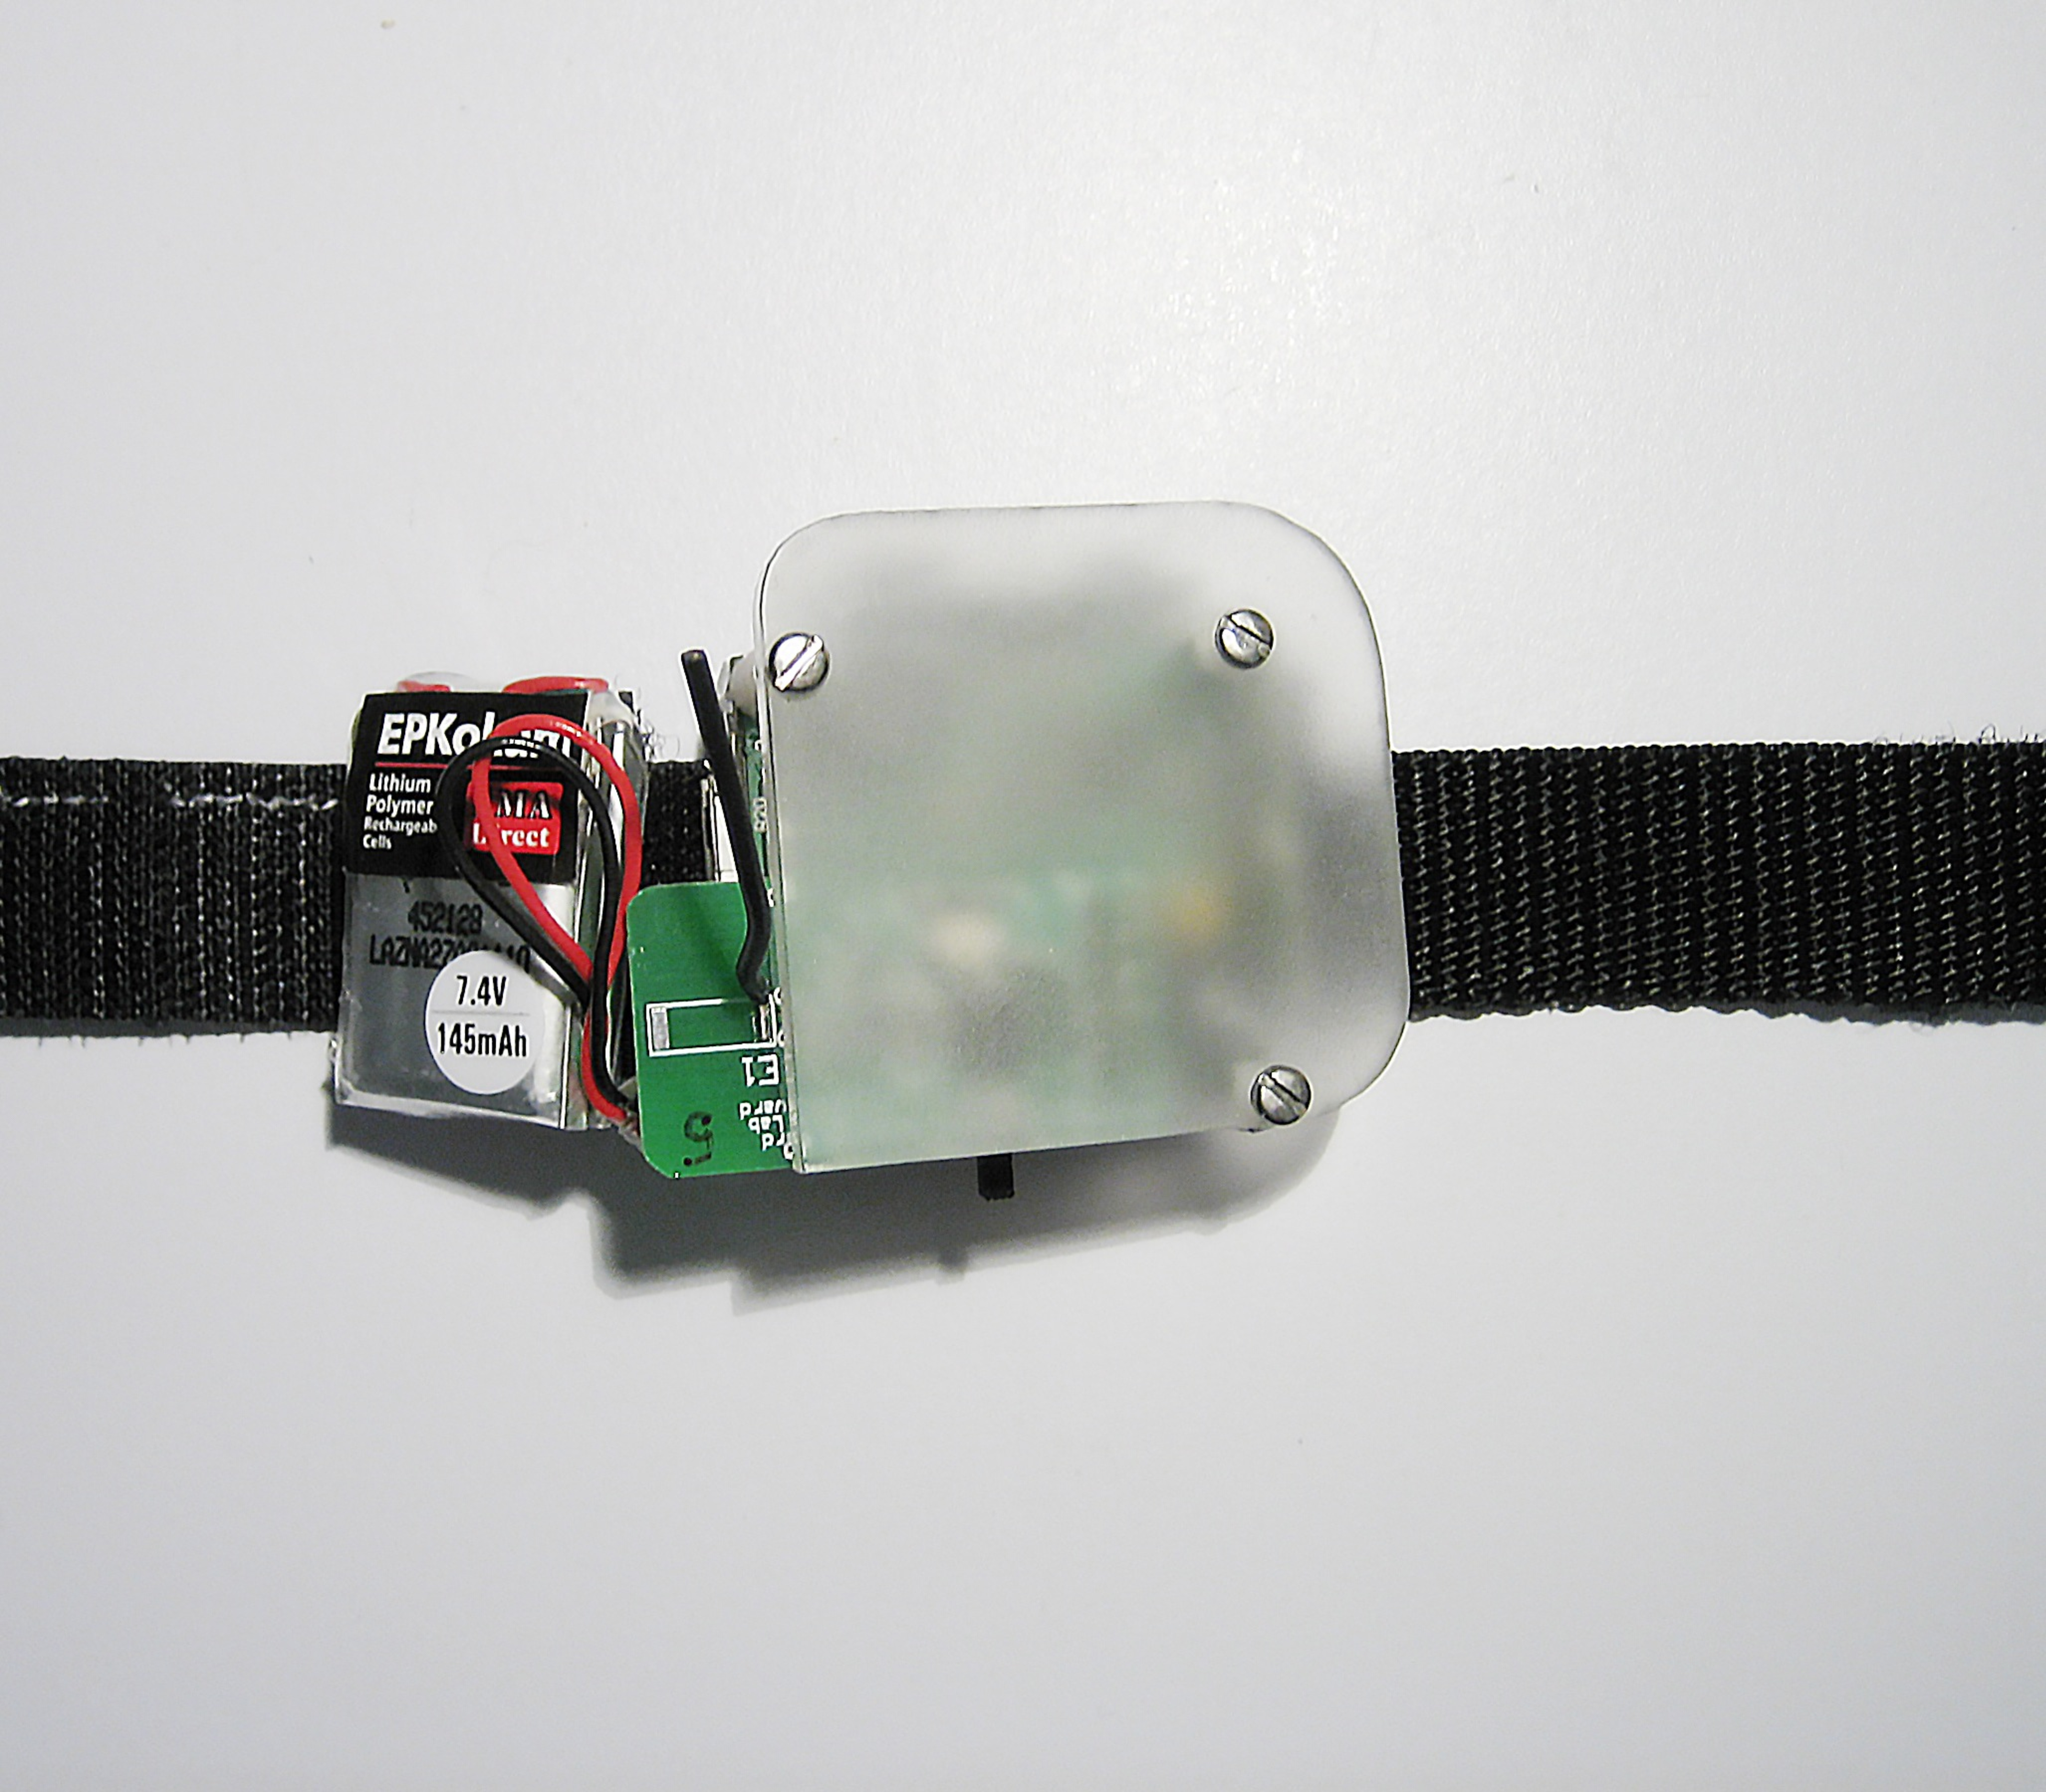
\includegraphics[height=40mm]{jp_fig1b}
\includegraphics[height=50mm]{jp_fig1c}
\caption{Sensor node on wrist (upper left), removed (upper right), and exposed circuit board (bottom).}
\label{Aylward:fig:1} 
\end{figure}

 The IMU is made up of Analog Devices ADXRS300 rate gyros and ADXL203 accelerometers, as well as associated analog circuitry. Sensor signals are collected by the 12-bit analog to digital converter built into the onboard processor, a TI MSP430F14x. This microcontroller was favored because of its low power consumption, capable A/D, and ample I/O, as well as its use in several of our group's ongoing projects.

The node-to-node capacitive proximity sensor operates by alternating transmit and receive modes on each of the sensor nodes, with only one node transmitting at a time, while the body is grounded. Because of timing constraints, it is not feasible to record measurements for every pair of nodes; rather, several simultaneous transmit nodes and several concurrent receive nodes can be selected in software. During transmit mode, the microcontroller drives an LC oscillator, which generates a high amplitude pulse (tens of volts peak-to-peak) at 91 kHz. During receive mode, the pulse is picked up by the receiving node, amplified, and sampled in quadrature to estimate its amplitude without the need for phase coherence. The nodes are able to use the same electrode for both transmit and receive modes, thanks to an efficient amplifier circuit inspired by the School of Fish, an electric field sensing tool designed several years ago by a former Media Lab student \cite{Smith:1999}. Capacitive sensing requires an electrode with sizeable area---this could possibly be integrated into the strap securing the sensor package to the body using highly conductive textiles such as Bekiweave.%\footnote{\url{http://www.bekaert.com/bft}}

Additional capabilities include a free digital input for interfacing with a
Polar heart rate monitor, a free SPI interface for connecting with other digital
devices, and a free analog input with associated signal conditioning circuitry
for handling an additional resistive sensor, such as a pressure sensor, bend
sensor, or light sensor. All of these optional signal lines are broken out to a
compact expansion port, which also acts as the programming interface.

Power consumption is always of prime importance in the design of wireless
devices; the power source tends to be the largest and most cumbersome component
of the system. Unfortunately, our desire to operate continuously with three rate
gyros prevents this design from meeting traditional low-power requirements. Each
gyro may consume up to 30mW, and their slow setup time prevents them from being
power cycled. The data radio is also comparatively power hungry, consuming up to
60mW in receive mode and 40mW in transmit mode, but this can be managed in code
by minimizing the amount of time spent in active modes. Ultimately, we chose to
operate the system with lithium polymer batteries because they are lightweight,
compact, and rechargeable. With two compact 145mAh cells in series, as pictured
in Figure~\ref{Aylward:fig:1}, the node can operate for four hours on one charge.

\begin{figure}[t]
\centering
\includegraphics[width=\textwidth]{jp_fig2} 
\caption{Raw data for hands raised and lowered in sequence (only the pitch gyro is shown) and resulting average cross-covariance.}
\label{Aylward:fig:2} 
\end{figure}

\section{Results}


The major advantage of having enough bandwidth to operate multiple sense points
on multiple wearers simultaneously is the ability to obtain detailed information
about correlated activity within a group. In the context of a dance ensemble,
time and spatial correlations can be used to determine which dancers are moving
together, which groups are leading or lagging, or perhaps which dancers are
responding to one another with complementary movements. With this in mind, our
preliminary analysis focuses mainly on the feasibility of extracting simple
features that can be used to describe general group dynamics.

\begin{figure}[t]
\centering
\includegraphics[width=100mm]{jp_fig3} 
\caption{Selected raw data from the ankles of three ballet students
performing a sequence of leg swings in unison.}
\label{Aylward:fig:3} 
\end{figure}

\subsection{Correlated Motion}


Previous work has shown that cross-covariance can be used to express both time
separation and spatial similarity of gestures performed by multiple users \cite{Aylward:2006a}.
For example, Figure~\ref{Aylward:fig:2} illustrates pitch gyro data for the hands of three subjects
performing a similar gesture in sequence. The locations of the peaks in the
associated cross-covariance curves (calculated with respect to subject 1) give
the time lags between the three events. In addition, the height of a peak gives a
measure of how well the signal shapes are correlated. In this way, we can also
obtain a sense for the spatial similarity of the events. Here, subject two does a
slightly better job at mimicking the motion of subject one.

One problem with cross-covariance as a feature is that it requires a complete
segment of data to calculate.  In a streaming situation, windowed
cross-covariance must be used, where the window size is chosen to make a tradeoff
between latency and the maximum time separation that can be expressed. A feasible
use of cross-covariance requiring a short window might be to follow how closely
dancers synchronize to music or to a leader, where the delays between their
correlated motions are expected to be within a second.

To test this idea, six sensors were given to three dancers participating in a
ballet lesson; each wore one on the right wrist and one on the right ankle. The
class then performed an exercise involving a repeated sequence of leg swings
executed in unison, to music.  Although they were roughly in time with the music,
the dancers were not necessarily looking at each other or at an instructor,
creating a small but clearly visible delay in their motions (the rehearsal was
documented on video for reference).  Figure~\ref{Aylward:fig:3} shows a portion of the raw data
collected from the leg of each dancer.  Because there was very little arm motion
associated with this exercise, only leg motion is discussed here. The area from
about 35 to 65 seconds corresponds to the synchronized sequence of swings made
with the right leg.

Figure~\ref{Aylward:fig:4} shows the result of windowed cross-covariance analysis on this data
segment with a window size of 1 second and a step size of 0.25 seconds. That is
to say, at each interval of 0.25 seconds, a window of data was considered, the
cross-covariance vector was computed individually for each sensor value, and then
the individual vectors were averaged to produce a result. Note that the area of
peak cross-covariance, shown in white, tends to waver around the baseline as time
progresses. This is consistent with the dancers slowly leading and lagging with
respect to one another by small amounts. Because the step size is small enough,
individual leg swings and their synchronicity across the ensemble can be picked
out. It is clear from the relatively stable middle plot that Dancer A and Dancer
C were closely synchronized for the duration of the exercise, while Dancer B
fluctuated from about 0.3 seconds ahead of Dancer A to 0.3 seconds behind Dancer
A. This fluctuation reflects accurately what is visible in the video.
Interestingly, it turns out that Dancers A and C were facing each other during
the exercise, while Dancer B had her back turned to the others.


\begin{figure}[t]
\centering
\includegraphics[width=100mm]{jp_fig4} 
\caption{Windowed cross-covariance (averaged across sensor values)
between pairs of dancers, for the data segment presented in Figure 3.}
\label{Aylward:fig:4} 
\end{figure}

\begin{figure}[t]
\centering
\includegraphics[width=100mm]{jp_fig5} 
\caption{Selected data and resulting activity envelopes as dancer
transitions from slow kicks to rapid tense kicks. Sequence of leg motions is
framed by stylistic arm motion.}
\label{Aylward:fig:5} 
\end{figure}


\subsection{Quantifying Activity}


In addition to extracting correlations between the activities of a group, it is
important to obtain information about the properties of the activities being
observed. These properties might include variations in the overall activity level
of an individual or group at different time scales, principal axes of movement,
or other features extracted during an interval of high activity.

One approach to activity measurement involves computing the average running
variance for various combinations of sensors on individual nodes. If the
separation between gestures is long enough, variance spikes can be used to
delineate them.  In other cases it might be useful to use a lowpass filter to
obtain an envelope on the running variance, in order to determine slower trends
in the activity level. For example, data was collected from the right wrist and
ankle of a ballet student performing a sequence of motions in which slow kicks
with the right foot transitioned into fast, tense kicks (in ballet terminology,
petit battement). The full sequence is framed with a stylistic tension and
release of the right arm at the beginning and end, respectively.  Figure~\ref{Aylward:fig:5} shows
a portion of the raw data from this segment along with four different activity
envelopes obtained from the windowed variance of both upper and lower body
movement. Accelerometer activity here denotes the average variance across the
accelerometer axes, while rotational activity denotes the average across the gyro
axes. One can clearly see a marked increase in activity as leg motion transitions
to faster kicking. The role of the arm movement is apparent in the activity
envelope as well.

\begin{figure}[t]
\centering
\includegraphics[width=100mm]{jp_fig6} 
\caption{Activity envelopes for the synchronized leg movement
highlighted in Figures 3 and 4.}
\label{Aylward:fig:6} 
\end{figure}

Similar conclusions can be drawn from Figure~\ref{Aylward:fig:6}, which illustrates the activity
envelopes of leg motion for each dancer during the period of correlated activity
highlighted earlier in figures 3 and 4.  Two areas of peak activity across the
ensemble appear around 50 and 60 seconds into the sample, corresponding to
repeated leg swings over the full range of motion from front to back and back to
front.  The general trend of activity is increasing over the segment from 30
seconds to 60 seconds, as the instructor urges the dancers to make each leg swing
``successively higher.''  Finally, we see activity for Dancer B in the interval
from 10 to 20 seconds that is not reflected in the movements of the other
dancers, corresponding to a few ``warm-up'' leg swings by Dancer B. Comparison of
the activity levels is all that is required to flag this unique period of
activity, at which point it could be analyzed more closely, or used as evidence
that Dancer B should be clustered in a different subgroup from Dancers A and C.
Note that the cross-covariance analysis shown in Figure~\ref{Aylward:fig:4} is unable to compare
the warm-up leg swings with motion occurring later in time, because the window is
only 1 second long. Given enough storage and computing power, one solution is to
save interesting data segments for correlation with future data, or to monitor
running cross-covariance on multiple time scales.

Looking at Figure~\ref{Aylward:fig:5} and \ref{Aylward:fig:6}, it would seem as if there is no reason to distinguish
between accelerometer and gyro activity. Indeed, sensor activity on a single node
is often highly correlated, because human motion is unlikely to occur along only
one axis. The accelerometers are also subject to gravity and centripetal
acceleration, so rotations will be picked up strongly in some cases. It should be
possible to use the gyro signals to help isolate translational acceleration from
other types of movement picked up by the accelerometers. However, if one wishes
to identify specific classes of activity, it may be more important to compare
motion along each axis than rotational versus translational motion. One approach
is to keep track of which sensor has the highest variance on each node or on each
individual, with the goal of analyzing activity one person at a time.  A more
efficient approach might be to create a group feature such as mean activity on
each sensor axis, for each limb, across the entire ensemble, to determine the
predominate axes of collective motion.

For example, Figure~\ref{Aylward:fig:7} demonstrates the results of a group of three people
raising and lowering their right hands in unison. The bottommost plot indicates
the variance on each sensor axis for the right arm, averaged across all three
subjects. Note that the average variance of the pitch gyro dominates. This
supports our intuition that the act of raising and lowering the hand involves
mostly a rotation in pitch. Extracting this information from average windowed
variance may simplify the task of detecting specific gestures by determining
which sensor signals are most important, or by defining a subgroup that is
performing a similar gesture before applying heavier analytical techniques. One
can also imagine a situation in which the correlation measurements discussed
above are desired, but it is unclear who should be interpreted reasonably as a
``reference'' for the rest of the group. By comparing the average group variance
to the individual variance, one can determine if the motions of a specific
subject are characteristic of the entire group, or lie outside the norm.

\begin{figure}[t]
\centering
\includegraphics[width=100mm]{jp_fig7} 
\caption{Right arm pitch gyro signals and windowed variance averaged
across subjects for each sensor axis, as hands are raised and lowered in unison.}
\label{Aylward:fig:7} 
\end{figure}

\subsection{Capacitive Sensor}


One of the limitations of small-scale inertial sensing is that it is extremely
difficult to obtain a reference frame for any sort of position tracking. Yet, the
shape of the body may be a more intuitive communication tool than the dynamics of
the body.  To supplement inertial data with information even as simple as ``arms
together'' and ``arms apart'' would add significant depth to the interface. This
was the idea behind the node-to-node capacitive proximity sensor.

Initial performance evaluations have determined that the capacitive system
suffers from a very nonlinear response, which, coupled with high noise levels,
limits its useful range (Figure~\ref{Aylward:fig:8}). Despite this, nodes grounded through the user's
body can be sensed up to a spacing of 30cm with a 16cm$^{2}$ electrode. Nodes
that do not share a ground, i.e. worn by different individuals, have reduced
range but can still be detected. Past attempts at similar sensing systems have
achieved better range, possibly due to higher voltage output on the transmitting
electrode \cite{Paradiso:1997b,Smith:1999}. It may thus be possible to improve the performance with minor
adjustments.

\begin{figure}[t]
\centering
\includegraphics[width=100mm]{jp_fig8} 
\caption{Typical response of the capacitive sensing system.}
\label{Aylward:fig:8} 
\end{figure}

In the current version, because of the reduced sensitivity beyond about 5cm, it
may not be efficient to transmit a full 12-bit value for every capacitive
measurement. Rather, the signal should be compressed to fit a range of 8 or fewer
bits with a more linear response. Another possibility is to use the existing
response to form a simple one-bit indication of close versus distant. Until
improvements can be made, this scheme fulfils the minimum requirements. In
either case, data reduction will enable the transmission of capacitive
measurements from more nodes without compromising the bandwidth available for
higher priority sensor data.

\section{Generating Musical Feedback}


To demonstrate the utility of the system as a multi-user interface for
interactive performance, it will be necessary to map extracted activity features
to musical sound in a satisfying way. In a traditional free gesture interface,
each degree of freedom might be mapped directly to a specific continuous control
or set of event triggers. In this system, however, there are at least six degrees
of freedom per node provided by the inertial sensors, and typically four nodes
per user, making direct mapping impractical. Taking the first step towards a
practical strategy for musical mapping in this framework, we have been focusing
on forming descriptions of motion at the group level rather than at the
individual level. As suggested above, simple group features can express a whole
range of useful information, such as who is leading and who is following, degree
of correlation across the ensemble, changes in activity level across the
ensemble, the existence of subgroups or clusters within the ensemble that could
be considered separately, principal axes of activity within subgroups, the
location of an event unique to one individual, or relationships between levels of
upper body motion and lower body motion.  In turn, the treatment of the ensemble
as an organic unit offers new possibilities for musical interpretation.

However, the potential amount of information expressed by these group features
alone is still too large for a direct mapping to music.  The problem can be
simplified by interpreting group dynamics in the context of a specific piece. For
example, the music can be generated from a loose framework or score designed
alongside the choreography. At a given point in the score, one may be looking for
a specific set of possible changes in the dancers' movements that signal musical
events such as changing timbral qualities, the entrance of a new melodic line, or
a shift to a new section. By placing contextual limits on the decision space,
pattern recognition algorithms can be trained on a specific performance to
streamline the control process. Although the dancers do not actually generate
music directly under this model, they are able to freely control their
progression through sections of the score, alter their interpretation of the
context, and add embellishments. This approach should provide a balance between
musical continuity and the sense of causality between the movements of the
dancers and the generated sound, which is essential for an engaging interactive
performance.

One limitation to address is the fact that many of the features discussed in
this paper are slowly varying, or have a significant amount of latency associated
with them. This is unsuitable for triggering sudden events or percussive sounds,
as the human tolerance to latency in this case is quite low. It may be possible
to train a state-based gesture-tracking model that would allow for rapid activity
detection by predicting future states, but applying a simple threshold on one or
more continuous features may be a better option.

\section{Conclusions \& Future Work}


In this paper, we have presented a compact, wearable sensor system enabling real
time collective activity tracking for interactive dance. The sensor node
comprises a full 6-axis inertial measurement unit with supplementary capacitive
node-to-node proximity sensing. Preliminary results demonstrate that our design
is viable for analyzing a wide range of collective activity parameters in a dance
setting. As the current $\pm{}$1.7g accelerometer was found to have insufficient
range to capture certain quick motions, it will be replaced by the $\pm{}$10g
ADXL210E. We also hope to increase the range of the capacitive sensor. Future
work will focus on adding to the feature set developed here, assessing real-time
operation with special attention to low-latency requirements, and developing a
more specific framework for music generation with implementations in Max/MSP or
PD.

\section*{Author Commentary: Doing Wireless Wearable Sensing Before the Internet of Things}
\paragraph{Joseph A. Paradiso}

After designing wearable wireless sensor nodes for interactive dance shoes in the late 90s \cite{Paradiso:2002} and gait analysis in the early 2000s \cite{Bamberg:2008}, I became interested in capture of real-time gestural features from multiple points on the bodies of an entire dance ensemble.  Although I sketched this by 2001 \cite{Paradiso:2002}, radios to do this weren't yet available.  For the original shoe system, we used small 20 kbps transmitters, streaming full-tilt from each shoe at different (and not entirely legal) frequencies.  We implemented a simple TDMA channel-sharing protocol for the Gait Shoe, but there wasn't nearly enough bandwidth to instrument arms and legs of a single dancer at 100 Hz updates, let along a troupe of 5, which was our goal.  Early Bluetooth chips that began to be available allowed only 8 nodes per piconet (we needed 20), and WiFi was bulky and power-hungry---these solutions implied latency issues as well, which challenged live performance.

By the mid-2000s, integrated, high-speed, programmable chip-based radios appeared \cite{Laibowitz:2004}.  Now, we could make a compact, wrist-or-ankle-worn module in the form-factor of a watch that could stream real-time data fast enough for our goals.  There were no protocols available \lq off-the-shelf\rq for the radios that could do real-time channel-sharing at these rates, so we designed our own.  Sensors were becoming increasingly integrated, but multi-axis inertial sensing was still nascent---we needed to employ two orthogonal breakout boards for 6-axis inertial sensing (done with a single chip routinely now and at much lower power).  We also implemented a capacitive pulsing scheme into our timing chain that enabled the proximity of any two devices to be inferred, although this required a large copper electrode around the wrist, giving it something of a \lq retro-Sci-Fi\rq look.

We picked a suite of correlation and kinematic features that could be extracted from the sensor stream in real-time.  We considered machine learning or detection of specific gestures, but were concerned about robustness in live performance.  We built 20 sensor nodes to capture the arm/leg motion of 5 dancers practicing, then subsequently ran this data through real-time feature-extraction and musical mapping.  Although this wasn't an end-end live performance, it demonstrated all components working together at the speeds needed for this.\footnote{Video: \url{http://www.media.mit.edu/~joep/MPEGs/Sensemble-Demo.mov}}  The following year (2007), we planned a performance at MIT's Kresge Auditorium.  We recruited a dance ensemble to choreograph a short routine, and wrote an elaborate MIDI mapping system to easily adapt musical events to the detected features.  Things worked in small practice rooms, but utterly failed in the large auditorium, as our little 2.4 GHz Nordic radios had problems transmitting through the body, which absorbs RF at that frequency.  If the dancers were facing the base station, the telemetry was fine.  When they turned away, the bit error rate became intolerable.  In our small practice room, we got sufficient signal because of reflection from the walls.  In the large open theatre, the multipath was too weak, hence as we lost the direct signal when going through the body, reception effectively ceased.

Before we could fix the radios and attempt another performance, we became derailed when the doctors for Boston's famous baseball team (the \lq Red Sox\rq) approached us about adapting our system for real-time multi-point biomotion capture of professional pitchers and hitters.  We made a set of Sensemble units with very high-range accelerometers and gyros to accommodate the extreme motion typical of these athletes at peak exertion, and brought it to Spring Training to take initial data.  This led to a multi-year collaboration and successive design refinements that pioneered wireless wearable inertial systems for high-intensity sports \cite{Lapinski:2009}.

In 2015, wireless sensing is ubiquitous, and many of us are wearing wireless IMUs on our wrists as athletic fitness bands or smart watches.  Although outfitting an entire dance ensemble with high-data-rate wireless sensors at all of their limbs isn't entirely off-the-shelf yet, systems begin to appear in the form of wireless nodes for multipoint motion capture.\footnote{For example, \url{http://www.xsens.com/} and \url{http://www.yeitechnology.com/}}  It's now turnkey to integrate a single-chip processor and Bluetooth radio into a sensor node, providing access to over 2 Mbs of aggregate bandwidth.  And smart radios of all sorts from many manufacturers are available from common online electronic retail stores. Real-time processing of live sensor streams has become even simpler, and machine-learning packages for dealing with sensor-derived gesture recognition are available, even customized for musical control \cite{Gillian:2014}.  But this paper shows how we did it when the Internet of Things was but a glimmer in Weiser's wake.


\section*{Expert Commentary: Wireless is paradise (compared to wires)}
\paragraph{Frederic Bevilacqua and Emmanuel Fl\'ety}

Perry Cook warned at the first NIME in 2001, in his well-known NIME proceeding on ``Principles for Designing Computer Music Controllers,'' about the difficulties in using wireless technologies. As he admitted later in 2007 at his keynote, this significantly changed over time. In 2015, wireless technologies are definitely anchored in the NIME community \cite{Mitchell:2014}. In this regards, the paper of Aylward \& Paradiso is certainly one of the key contribution that paved the way for using compact multi-user wireless technologies in the NIME community.


Even if the wireless technologies have greatly evolved over the last ten years \cite{Flety:2011}, Aylward \& Paradiso's contribution remains impressive today. The paper is still very informative. First, it provides some important references in movement capture technologies used in the performing arts prior to 2006. 

For example, it is important to keep in mind that wireless technologies had already successively been used in the 90's in the performing arts, while it was still rudimentary compared what Aylward \& Paradiso described in this NIME paper. Second, the hardware design is still worth reading for everyone willing to implement wireless sensor systems. In particular, the paper clearly states the constraints in term of frequency update of the system, number of units and the necessary bandwidth. Overall, the general architecture of the system represents a good example of compromising between all the constraints, also including battery consumption and size.

Though the trend was already to move to the CSMA/CA (collision avoidance transmission scheme (as in WiFi and Zigbee protocols), the system both features a high data rate, enough for a fair amount of performers, and TDMA (Time Division Multiple Access) to achieve a better, synched transmission of the sensor nodes by minimizing the latency jitter. This is particularly important since jitter latency has been shown to degrade real-time high resolution sensor signal streams, possibly more than lowering sampling resolution [Schmeder and Freed 2008].

The description of the sensors analysis is also interesting. The use of inertial measurement units, here 6 DoF (degrees of freedom) with accelerometers and gyroscopes, is another point that have been broadly accepted over the years. They proposed both an analysis based on correlation measured and on an average activity measure. Most importantly, they proposed to analyze dancer's activities from a group perspective instead of each individual dancer. Such an analysis using inertial
measurement units still represent today a challenge that is also shared by other recent communities such as social computing.

The collective interaction aspect described in this paper represents indeed another visionary aspect of this work. As already mentioned, the technical aspects related to wireless sensing has been largely addressed by the NIME community in the following years of this paper, and it is much easier today to develop and/or access to wireless system with of-the–shelf technologies. Nevertheless, we believe that strong concepts and aesthetics behind ``collective interaction'' have still to emerge.

%\bibliographystyle{abbrv}
%\bibliography{nime_reader}

